\section{Objetivos}

Estimar os erros em regime permanente e identificar os parâmetros do kit Impressora. Deve-se comparar de forma critica os resultados estimados e os que eram esperados para o kit.

\section{Introdução}
Esta seção destina-se à breve descrição do kit impressora utilizado e introduzir os métodos de identificação de sistemas utilizado..

\subsection{Kit Impressora}
O kit impressora, desenvolvido pelo prof. Egito da Universidade de Brasília consiste na adaptação e instrumentação de uma impressora para análises de controle.  O esquemático de entradas e saídas do kit pode ser revisado em \cite{CDIN:Roteiro1}. O kit pode ser visualizado na Figura \ref{kit_impressora}.

\begin{figure}[ht]
	\begin{center}
		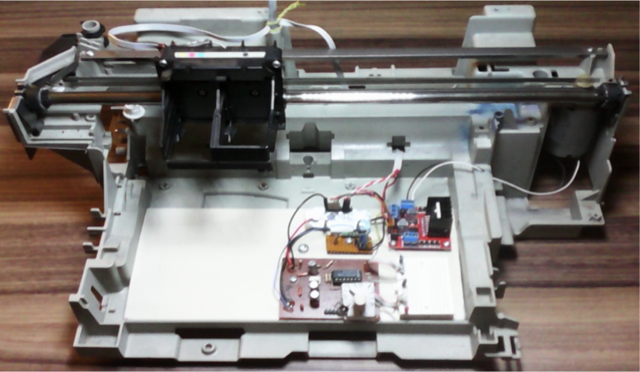
\includegraphics[width=\textwidth,keepaspectratio]{img/kit_impressora.png}
       \caption{Kit Impressora utilizado neste experimento. Desenvolvido pelo professor Egito do departamento de eng. elétrica da Universidade de Brasília. Fonte da imagem: \cite{CDIN:Roteiro1}.}
       \label{kit_impressora}
	\end{center}
\end{figure}

\subsubsection{Componentes}
O kit é composto de um motor  corrente contínua acoplado ao carro de cartuchos de tinta da impressora. O movimento do carro é realizado por um microcontrolador Arduíno Nano, que envia comandos por uma ponte H e monitora a posição do carro por meio de um Encoder. 

A placa de circuito impresso anexada embarca o amplificador de diferenças e amplificadores operacionais cujas entradas são ligadas à protoboard. Deve-se conectar o sinal de referências a esta placa. Na protoboard, deve-se realizar a montagem do circuito de controle, que relaciona o erro entre posição e sinal de referência com o sinal de controle que será enviado ao motor.

\subsection{Modelagem do Sistema}
O modelo do sistema pode ser simplificado no diagrama da Figura \ref{kit_modelagem}. Segundo \cite{CDIN:Roteiro1}: sendo $Y(S)$ a saída em posição do sistema e $R(S)$ o sinal de referência, a sua função de transferência pode ser expressa na equação \ref{eq::Y-R-model}.
\begin{equation}
% feita com https://www.codecogs.com/latex/eqneditor.php?lang=pt-br
\frac{Y(S)}{R(S)} = \frac{ K_p K K_m  }{ K_p K K_m + S(ST_m +1) } = \frac{\frac{K_p K K_m}{T_m}}{S^2+ \frac{S}{T_m}+ \frac{K_p K K_m}{T_m}} 
\label{eq::Y-R-model}
\end{equation}

Também é possível modelar a relação distúrbio, $W(S)$, e posição, $Y(S)$, no sistema. O roteiro \cite{CDIN:Roteiro1} descreve essa relação conforme expresso na equação \ref{Y-W-model}.

\begin{equation}
% feita com https://www.codecogs.com/latex/eqneditor.php?lang=pt-br
\frac{Y(S)}{R(S)} = \frac{ K K_m  }{ K_p K K_m + S(ST_m +1) } 
\label{Y-W-model}
\end{equation}

Nas equações \ref{eq::Y-R-model} e \ref{Y-W-model}, as constantes $K_p$, $K$ e $K_m$ representam o ganho do potenciômetro, o ganho do circuito de amplificação e o ganho do motor, respectivamente. O parâmetro $T_m$ é a constante de tempo do motor.

\begin{figure}[ht]
	\begin{center}
		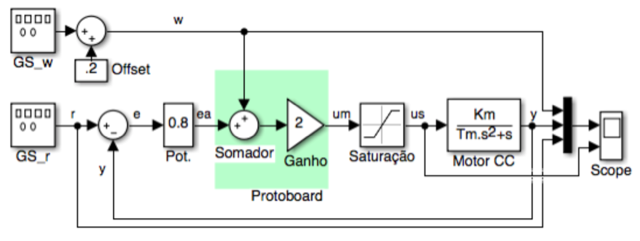
\includegraphics[width=\textwidth,keepaspectratio]{img/kit_blocos.png}
       \caption{Diagrama de blocos simplificado do kit impressora. Extraído de \cite{CDIN:Roteiro1}.}
       \label{kit_modelagem}
	\end{center}
\end{figure}


\subsection{Identificação de Sistemas de Segunda Ordem}
Neste experimento será realizada a identificação do sistema kit impressora como um sistema dinâmico de segunda ordem \cite{Nise:ControlSistemsEngineering}. Esse tipo de sistema pode ser modelado conforme a equação \ref{eq::second-order-model}.

\begin{equation}
% feita com https://www.codecogs.com/latex/eqneditor.php?lang=pt-br
G(S) = \frac{Y(S)}{R(S)} = \frac{ \omega_n ^2  }{ S^2 + 2 \zeta \omega_n S + \omega_n ^2 } 
\label{eq::second-order-model}
\end{equation}

A partir do modelo da planta kit impressora, representado na equação \ref{eq::Y-R-model} e da resposta esperada do sistema da equação \ref{eq::second-order-model}, pode-se fazer uma relação entre os coeficientes da planta e a resposta do sistema. Essa relação está expressa na equação \ref{eq::comparison-second-order-plant}

\begin{equation}
\begin{aligned}
\frac{Y(S)}{R(S)} ={} & \frac{ \omega_n ^2  }{ S^2 + 2 \zeta \omega_n S + \omega_n ^2 } = \frac{\frac{K_p K K_m}{T_m}}{S^2+ \frac{S}{T_m}+ \frac{K_p K K_m}{T_m}} \\
& \omega_n ^2 = \frac{K_p K K_m}{T_m} \\
& \zeta = \frac{1}{2\sqrt{T_m K_m K_p K}}
\end{aligned}
\label{eq::comparison-second-order-plant}
\end{equation}

Dessa maneira, podemos estimar os parâmetros da planta: $K_p$, $K$, $K_m$ e $T_m$ a partir da resposta do sistema de segunda ordem registrada em laboratório.

O coeficiente de amortecimento $\zeta$ e a frequência natural podem ser estimados a partir do sobressinal ($OS$) registrado e do tempo de pico ($t_p$), respectivamente \cite{ogata2003engenharia}. Suas relações estão expressas nas equações \ref{eq-zeta} e \ref{eq-tempo-pico}.

\begin{equation}
\zeta = \frac{\ln(OS)}{\sqrt{\pi^2 + \ln(OS)^2}}
\label{eq-zeta}
\end{equation}

\begin{equation}
\omega_n = \frac{\pi}{t_p}
\label{eq-tempo-pico}
\end{equation}

Vale lembrar que, por definição \cite{Nise:ControlSistemsEngineering}, o sobressinal $(OS)$ pode ser expresso conforme a equação \ref{eq-Sobressinal}, em que $V_p$ é a tensão de pico e $G_{ss}$ é a resposta em regime permanente do sistema.

\begin{equation}
OS = \frac{V_p - G_{ss}}{G_{ss}}
\label{eq-Sobressinal}
\end{equation}

\subsection{Erro em Regime Permanente}
Ao buscar-se que o erro seja o mais próximo possível do zero, é necessário a colocação de um integrador na malha. A partir desse integrador, o sistema passará a ser capaz de acompanhar o sinal de entrada, porém agora com um erro finito. O erro em regime permanente representa o erro que um sistema apresenta após a sua fase transitória ter acabado.
O erro é definido como o 
\begin{equation}
    Referencia - Erro
\end{equation}
E, para se encontrar o erro em regime permanente, basta aplicar-se o teorema do valor final. Ao se calcular a função de transferência em malha aberta, basta observar o grau $N$ do polinômio do divisor.


\subsection{Tipo de Sistemas}
A classificação dos sistemas de controle é dada de acordo com a sua habilidade em seguir sinais de entrada. Tais sinais podem são dos mais variados tipos como degrau, rampa, parábola entre outros. A qualidade desses sistemas é indicada pelos valores dos erros estacionários que são apresentados por estas entradas.
Desta forma, os tipos de sistemas são nomeados de acordo com o número de integradores que encontram-se na função de transferência em malha aberta.
Os tipos são:
\begin{itemize}
    \item Tipo 0: Não apresenta nenhum integrador
    \item Tipo 1: Apresenta um integrador
    \item Tipo 2: Apresenta dois integradores
\end{itemize}

